% This is samplepaper.tex, a sample chapter demonstrating the
% LLNCS macro package for Springer Computer Science proceedings;
% Version 2.20 of 2017/10/04
%
\documentclass[runningheads]{llncs}
%
\usepackage{graphicx}
\usepackage[spanish]{babel}
\usepackage[utf8]{inputenc}
% Used for displaying a sample figure. If possible, figure files should
% be included in EPS format.
%
% If you use the hyperref package, please uncomment the following line
% to display URLs in blue roman font according to Springer's eBook style:
% \renewcommand\UrlFont{\color{blue}\rmfamily}

\begin{document}
%
\title{Motor de Búsqueda}
%
%\titlerunning{Abbreviated paper title}
% If the paper title is too long for the running head, you can set
% an abbreviated paper title here
%
\author{Luis Ernesto Ibarra Vázquez\inst{1} \and
Luis Enrique Dalmau Coopat\inst{2} \and
Adrian Hernández Pérez\inst{3}}
%
\authorrunning{Luis Ibarra, Luis Dalmau, Adrian Hernández}
% First names are abbreviated in the running head.
% If there are more than two authors, 'et al.' is used.
%
\institute{Universidad de La Habana, La Habana, Cuba\\
\url{https://www.uh.cu}}
%
\maketitle              % typeset the header of the contribution
%
\begin{abstract}
% The abstract should briefly summarize the contents of the paper in
% 150--250 words.
La creación de motores de búsqueda permiten a los usuarios acceder a la información
que buscan de manera rápida y eficiente. Este trabajo presenta una implementación de 
un motor de búsqueda basado en el modelo vectorial. Se presentan la arquitectura,
algoritmos y procesamientos usados para dicha implementación. Se obtuvieron resultados ...
%TODO PONER RESUMEN DE RESULTADOS

El resultado final es presentado al usuario mediante una interfaz gráfica que permite
al usuario realizar consultas de manera natural.

\keywords{Recuperación de Información  \and Motor de Búsqueda \and Modelo Vectorial. \and SVM}
\end{abstract}

\section{Introducción}

El ámbito de recuperación de información es un área de las Ciencias de la Computación que tiene
actualmente gran importancia debido al gran volumen de información que se genera cada día en la
web. Esta información debe de ser encontrada por los usuarios de manera rápida y eficiente y es
de esta tarea en la cual un motor de búsqueda es necesario. La tarea escencial de un motor de
búsqueda es la de recuperar documentos que estén asociados a una pregunta planteada por el usuario, 
esta recuperación tiene que ser de calidad conteniendo información relevante que el usuario pueda
usar para lograr su objetivo.

En este ámbito se presentan escencialmente tres tipos de modelos de recuperación de los
cuales surgen nuevas variantes, los tipos son:

\begin{itemize}
    \item Vectorial
    \item Probabilístico
    \item Booleano
\end{itemize}

El objetivo del trabajo consiste en la implementación y evaluación de un motor de búsqueda,
en este caso se usa el modelo vectorial y el modelo de Ranking SVM. Además es necesario la
construcción de una interfaz visual para la interacción con el usuario, en este caso se usó
streamlit y Flutter para la construcción de páginas web con esta finalidad.

El trabajo de divide en varias secciones, primero se analizará la arquitectura del motor de
búsqueda, luego se presentará el algoritmo y procesamiento usado para la implementación de 
este, luego se presentará el resultado final del motor de búsqueda. También se presentará una
sección sobre la implementación de la interfaz gráfica. 

\section{Arquitectura}

Todo motor de búsqueda consta de tres partes fundamentales a la hora de darle respuesta al usuario

\begin{itemize}
    \item Recibir una pregunta
    \item Buscar documentos relevantes a la pregunta
    \item Devolver los documentos relevantes encontrados
\end{itemize}

\subsection{Flujo de datos del motor de búsqueda}

El motor de búsqueda es el núcleo fundamental de la implementación. Un problema fundamental que
tiene la etapa de desarrolo es que en esta se realizan muchos cambios en el código fuente agregando
o cambiando funcionalidades al procesamiento, además estas funcionalidades generalmente se pueden usar
de manera independiente para otros procesamientos como por ejemplo la implementación de otro modelo
dentro del mismo motor de búsqueda. Para poder resolver este problema de una manera sencilla se estructura
el proyecto mediante una arquitectura de tuberías (pipelines). Esta arquitectura consiste en una serie
de tuberías que se conectan entre sí, pasando un contexto entre ellas y combinando de forma desacoplada
los resultados obtenidos de cada tubería. Un ejemplo de lo anterior es que la lectura de los documentos
es independiente de su procesamiento así que si se quiere cambiar esta funcionalidad es solamente necesario
cambiar el pedazo del pipeline encargado de esto, otro ejemplo de las ventajas es que el proceso de
tokenización de los documentos generalmente es el mismo, en el caso de que se quieran implementar varios
modelos se puede reutilizar este pipeline sin mucho esfuerzo y manteniendo la misma arquitectura \ref{pipeline_fig}.

\subsection{Comunicación con el motor de búsqueda}

La comunicación del motor de búsqueda con el exterior se hace a través de una API REST. Con esta
es posible preguntarle al motor de búsqueda y que este devuelva las respuestas asociadas. Gracias
a que la comunicación se hace mediante HTTP es posible realizar la implementación de varios clientes
que consuman de esta y que presenten la información de la manera que más le convenga al cliente.\\

Los principales endpoints de esta interfaz son:

\begin{itemize}
    \item GET \url{search/?query=query\&offset=offset} Devuelve una lista asociada a los
documentos relevanes de la búsqueda.
    \item GET \url{document/?document\_dir=document\_dir} Devuelve el contenido del documento asociado
al id dado.
	\item GET \url{expand/?query=query} Devuelve las posibles expansiones de query encontradas por el programa
	\item POST \url{feedback/} Envía la información para marcar como relevante o no los documentos mostrados.
\end{itemize}

\section{Implementación del motor de búsqueda}

\subsection{Tokenización}

La tokenización es el proceso en el cual se divide una cadena de caracteres en palabras o tokens.
Estos tokens son luego procesados en dependencia del modelo de búsqueda que se quiera implementar.
La implementación de la tokenización en el motor de búsqueda se lleva a cabo mediante el uso del
framework nltk. Esta es dividida principalmente en varias etapas:

\begin{enumerate}
    \item Convertir el texto en tokens
    \item Limpiar los tokens
    \item Remover las stopwords
    \item Aplicar stemming o lemmatizing a los tokens
\end{enumerate}

Mediante estos proceso se llega al final de esta etapa con una lista de tokens procesada la cual
representa el documento. Esta lista es luego convertida a la representación necesitada en cada modelo
para su procesamiento.

Este procesamiento puede ser el mismo independientemente del tipo de modelo utilizado.

\subsection{Modelo Vectorial}

El modelo vectorial se centra en la idea de que la relevancia de los documentos con la query está 
dada por las palabras que contienen. Para esto se encuentran representaciones vectoriales de ambos
para que se pueda hacer la comparación. En el modelo planteado en el trabajo se hace una implementación
del modelo clásico vectorial el cual no toma en cuenta el orden de las palabras en su representación, haciendo
de este un modelo estilo bolsa de palabras.

\subsubsection{Representación de los documentos}

Para el procesamiento del modelo vectorial se utiliza una representación de documentos en forma de
vectores. Esta representación se obtiene a partir de la tokenización previa de los documentos. La
representación de los documentos se obtiene a partir de la siguiente fórmula:

\begin{equation}
    w_{ij} = \frac{tf_{ij}}{\max_{k} tf_{kj}}idf_{j}
\end{equation}

Donde $w_{ij}$ representa el peso asociado al término $i$ en el documento $j$ y $tf_{ij}$ el número de veces que
se repite el término $i$ en el documento $j$. $idf_{j}$ es la frecuencia inversa del documento $j$ en la
colección de documentos calculada por $\log{\frac{N}{n_j}}$ donde $n_j$ es la cantidad de documentos
en donde aparece el término $j$.

\subsubsection{Representación de la pregunta}

La representación de la pregunta en el modelo vectorial es la misma que la representación de los 
documentos, pero con una diferencia que se aplica a la pregunta una fórmula diferente.

\begin{equation}
    (\alpha idf_i + (1-\alpha)\frac{tf_{ij}}{\max_{k} tf_{kj}}) idf_i
\end{equation}

En este caso $\alpha$ es un hiperparámetro para suavizar cuyo rol es disminuir
la contribución del segundo término \cite{alphaManning}.

\subsubsection{Ranking de documentos}

Para el ordenamiento de los documentos se utiliza la representación de la pregunta y de los documentos
en su forma vectorial. Para el cálculo de la similitud entre ambas se utiliza el coseno entre
ambos vectores:

\begin{equation}
    sim(q,d_i) = \cos(q, d_i) = \frac{q \cdot d_i}{||q|| ||d_i||}
\end{equation}

Una vez se tienen estos valores se ordenan de mayor a menor y son devueltos en ese orden al
usuario.

\subsection{Modelo Ranking SVM}

El modelo Ranking SVM se basa en que los documentos se pueden representar como vectores
en los cuales se guarda información acerca de sus características. Inicialmente un problema
el problema con que trata SVM es uno de clasificación, por lo que se tendría que convertir
el problema de Ranking a uno de clasificación. Para esto se considera la siguiente idea, se
entrenará el modelo SVM para detectar si un documento es más relevante a otro con la misma query.

\subsubsection{Representación de Documentos y Preguntas}

Dado que el modelo necesita tener información acerca de la pregunta y su relación con el documento
se modela una representación conjunta de ambos. Esta representación conjunta puede guardar todo tipo
de información aunque en el trabajo se representa por la concatenación de los siguientes aspectos:

\begin{itemize}
	\item Coseno entre la representación vectorial TF-IDF de la pregunta y el documento
	\item Cantidad de palabras que aparecen en la pregunta y el documento
	\item Representación reducida del vector TF-IDF de la pregunta mediante descomposición SVD
	\item Representación reducida del vector TF-IDF del documento mediante descomposición SVD
\end{itemize}

La descomposición de SVD se basa en el proceso de Latent Semantic Analysis (LSA) cuyo objetivo 
consiste en reducir la dimensionalidad de los términos aplicándole la descomposición SVD a la
matriz de TF-IDF generada en orden de obtener una representación más compacta y que guarde 
información semántica de los términos \cite{lsaWiki}.

\subsubsection{Ranking de los documentos}

Para la conversión del problema de ranking a uno de clasificación se parte de la siguiente
hipótesis en el espacio del trabajo con SVMs:

$$
w\theta_{iq} > w\theta_{jq} \iff r_q(d_i) > r_q(d_j)
$$

Donde:

\begin{itemize}

	\item $w$: Son los pesos encontrados de aplicar SVM al conjunto de entrenamiento
	\item $\theta_{iq}$: Es la representación conjunta del documento i con la query
	\item $r_q(d_i)$: Es la relevancia del documento i con respecto a la query
	
\end{itemize}

Partiendo de lo anterior se tiene que:

$$
w(\theta_{iq} - \theta_{jq}) > 0 \iff r_q(d_i) - r_q(d_j) > 0
$$

Lo que en términos de SVM equivale a encontrar el hiperplano que maximiza la distancia entre las distintas clases
del vector diferencia visto anteriormente.

\subsection{Retroalimentación}

Para la retroalimentación se eligió el algoritmo de Rocchio debido a su simplicidad. Este se basa 
en el cálculo de centroides de un conjunto de documentos relevantes y no relevantes a una query
y su posterior suma ponderada con el objetivo de mover el vector query hacia el conjunto de 
documentos relevantes y alejarlo del conjunto de documentos no relevantes. La fórmula final sería

\begin{equation}
    q_f = \alpha q_0 + \beta \frac{\sum_{d_r \in D_r} d_r}{|D_r|} - \gamma \frac{\sum_{d_{nr} \in D_{nr}} d_{nr}}{|D_{nr}|} 
\end{equation}

Dado que la relevancia depende de la query, se crea una estructura de datos la cual guarda esta correspondencia. 
En un principio esta estructura de datos solamente guarda los vectores relevantes o no que coincidan exactamente
con la query, aunque se pueden crear variantes de esta estructura que devuelvan los documentos relevantes o no
relevantes que estén en una zona cercana y no exacta aumentando así el recuperado de estos documentos.
%TODO Implementar esta última idea, ver qué funciona mejor y ponerlo en el informe

\subsection{Expansión de query}

%TODO Implementar
Implementar algoritmo de expnsión de query

\section{Interfaz gráfica}

La interfaz gráfica actúa como un cliente REST que consume los servicios de búsqueda. Esta
se presenta como un navegador web que le permite realizar todas las interacciones necesarias
con el motor de búsqueda \ref{ui_fig}.

Entre las acciones posibles a realizar se encuentran:

\begin{itemize}

\item Hacer una consulta.
\item Ver el contenido de un documento.
\item Dar feedback mediante like o dislike.
%TODO Mantener actualizada

\end{itemize}

Fue implementada en Flutter pudiendo ser compilada a varios sistemas operativos como Android,
iOS además de a web.

\section{Evaluación}

%TODO
Hablar del corpus de evaluación y exponer las métricas estudiadas y que tan bien se desempeña el
motor de búsqueda.

\section{Conclusiones}

%TODO
Hacer conclusiones
El modelo Vectorial pese a ser sencillo y obtener buenos resultados de manera sintactica, al probarse con el dataset de cranfield
presento problemas para la recuperación de informacion meramente semantica con respecto a una consulta. Consultas del tipo: "qué","como" 
y de ese estilo que requieren de una respuesta al significado semantico de la misma consulta.
La biblioteca de python cuenta con un TfidfVectorizer el cual nos da como resultado una matriz de TF*IDF del corpus de documentos
entregados como argumento a su metodo fit\_transform.
La consulta es pasada como argumento al metodo transform del mismo vectorizer ya ajustado al corpus de documentos, lo cual devuelve un
 vector normalizado de tf*idf de dicha consulta. Por tanto en el metodo smooth\_query donde deberia haber una multiplicacion de tf*idf 
 solo se encuentra query["vector"]. 


% \section{First Section}
% \subsection{A Subsection Sample}
% Please note that the first paragraph of a section or subsection is
% not indented. The first paragraph that follows a table, figure,
% equation etc. does not need an indent, either.

% Subsequent paragraphs, however, are indented.

% \subsubsection{Sample Heading (Third Level)} Only two levels of
% headings should be numbered. Lower level headings remain unnumbered;
% they are formatted as run-in headings.

% \paragraph{Sample Heading (Fourth Level)}
% The contribution should contain no more than four levels of
% headings. Table~\ref{tab1} gives a summary of all heading levels.

% \begin{table}
% \caption{Table captions should be placed above the
% tables.}\label{tab1}
% \begin{tabular}{|l|l|l|}
% \hline
% Heading level &  Example & Font size and style\\
% \hline
% Title (centered) &  {\Large\bfseries Lecture Notes} & 14 point, bold\\
% 1st-level heading &  {\large\bfseries 1 Introduction} & 12 point, bold\\
% 2nd-level heading & {\bfseries 2.1 Printing Area} & 10 point, bold\\
% 3rd-level heading & {\bfseries Run-in Heading in Bold.} Text follows & 10 point, bold\\
% 4th-level heading & {\itshape Lowest Level Heading.} Text follows & 10 point, italic\\
% \hline
% \end{tabular}
% \end{table}


% \noindent Displayed equations are centered and set on a separate
% line.
% \begin{equation}
% x + y = z
% \end{equation}
% Please try to avoid rasterized images for line-art diagrams and
% schemas. Whenever possible, use vector graphics instead (see
% Fig.~\ref{fig1}).

% \begin{figure}
% % 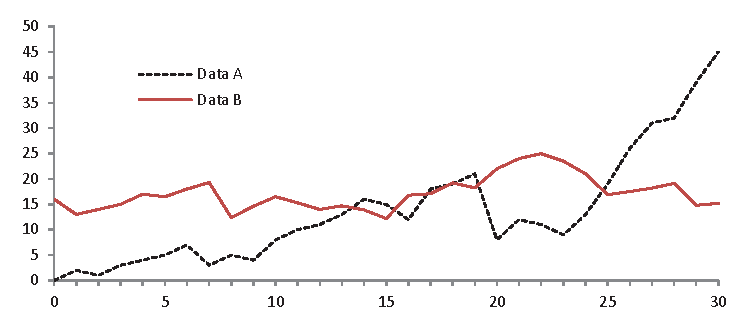
\includegraphics[width=\textwidth]{fig1.eps}
% \caption{A figure caption is always placed below the illustration.
% Please note that short captions are centered, while long ones are
% justified by the macro package automatically.} \label{fig1}
% \end{figure}

% \begin{theorem}
% This is a sample theorem. The run-in heading is set in bold, while
% the following text appears in italics. Definitions, lemmas,
% propositions, and corollaries are styled the same way.
% \end{theorem}
% %
% % the environments 'definition', 'lemma', 'proposition', 'corollary',
% % 'remark', and 'example' are defined in the LLNCS documentclass as well.
% %
% \begin{proof}
% Proofs, examples, and remarks have the initial word in italics,
% while the following text appears in normal font.
% \end{proof}
% For citations of references, we prefer the use of square brackets
% and consecutive numbers. Citations using labels or the author/year
% convention are also acceptable. The following bibliography provides
% a sample reference list with entries for journal
% articles~\cite{ref_article1}, an LNCS chapter~\cite{ref_lncs1}, a
% book~\cite{ref_book1}, proceedings without editors~\cite{ref_proc1},
% and a homepage~\cite{ref_url1}. Multiple citations are grouped
% \cite{ref_article1,ref_lncs1,ref_book1},
% \cite{ref_article1,ref_book1,ref_proc1,ref_url1}.
%
% ---- Bibliography ----
%
% BibTeX users should specify bibliography style 'splncs04'.
% References will then be sorted and formatted in the correct style.
%
% \bibliographystyle{splncs04}
% \bibliography{mybibliography}
%
\section{Anexos}

%TODO Poner ejemplo de como se puede reutilizar un pipeline para realizar otros pipelines
\begin{figure}
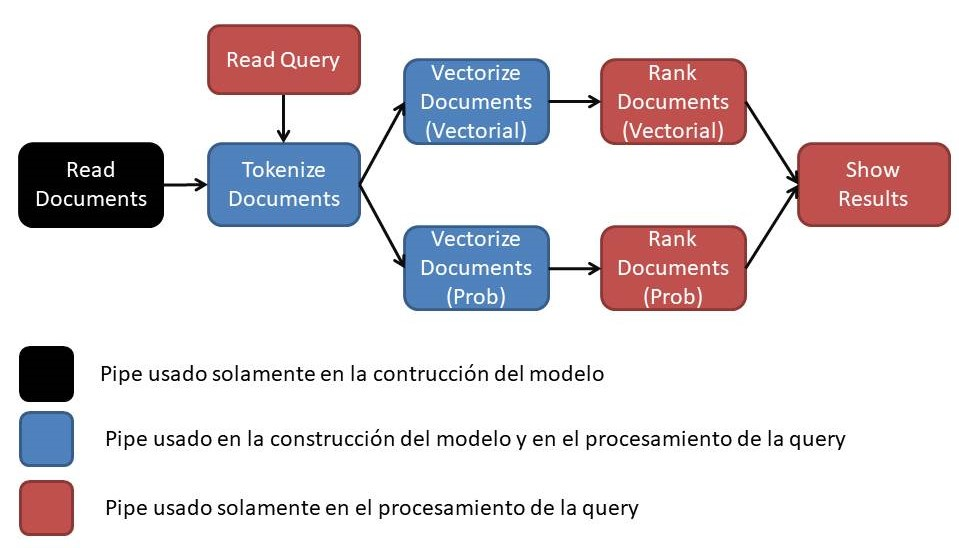
\includegraphics[width=\textwidth]{pipeline.jpg}
\caption{Ejemplo de pipelines} \label{pipeline_fig}
\end{figure}

\begin{figure}
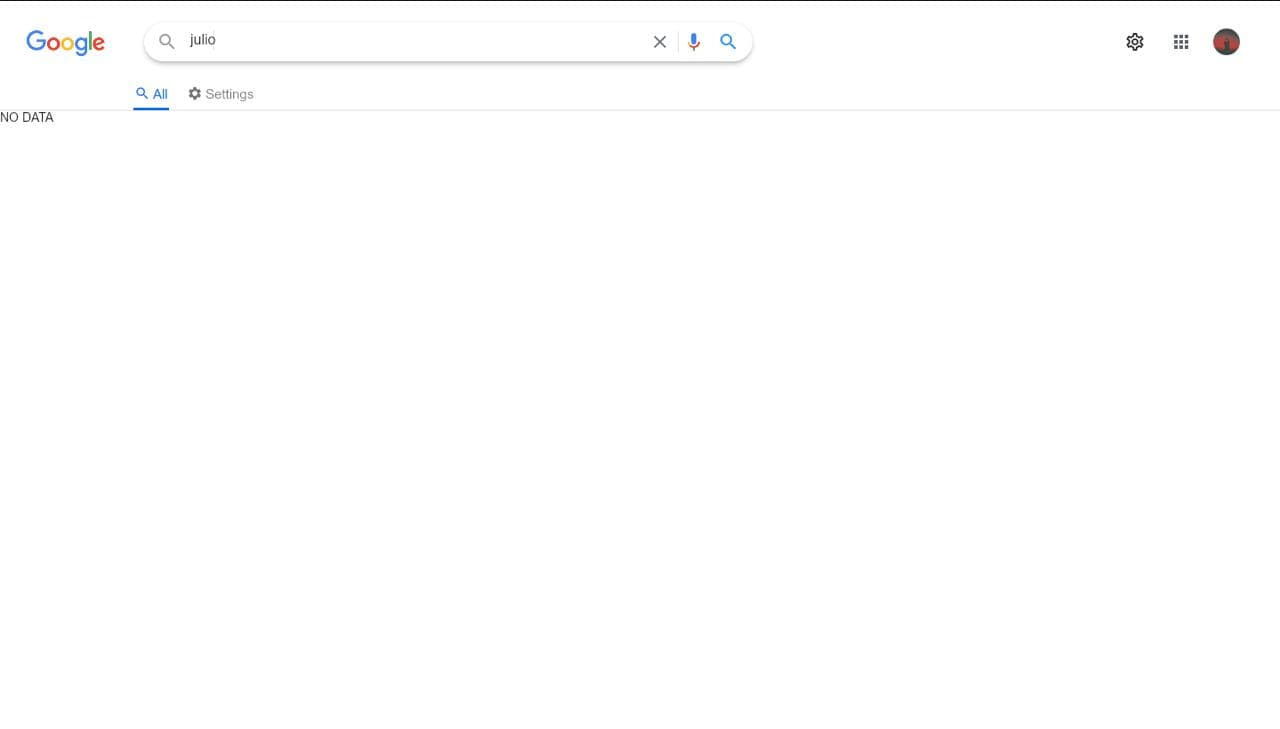
\includegraphics[width=\textwidth]{ui.jpg}
\caption{Interfaz visual} \label{ui_fig}
\end{figure}
    
\begin{thebibliography}{8}
% \bibitem{ref_article1}
% Author, F.: Article title. Journal \textbf{2}(5), 99--110 (2016)

% \bibitem{ref_lncs1}
% Author, F., Author, S.: Title of a proceedings paper. In: Editor,
% F., Editor, S. (eds.) CONFERENCE 2016, LNCS, vol. 9999, pp. 1--13.
% Springer, Heidelberg (2016). \doi{10.10007/1234567890}

% \bibitem{ref_book1}
% Author, F., Author, S., Author, T.: Book title. 2nd edn. Publisher,
% Location (1999)

% \bibitem{ref_proc1}
% Author, A.-B.: Contribution title. In: 9th International Proceedings
% on Proceedings, pp. 1--2. Publisher, Location (2010)

% \bibitem{ref_url1}
% LNCS Homepage, \url{http://www.springer.com/lncs}. Last accessed 4
% Oct 2017

\bibitem{alphaManning}
Christopher D. Manning, Prabhakar Raghavan, and Hinrich Schütze:
An Introduction to Information Retrieval. Online edition, pp. 127 Cambridge University Press,
Cambridge, England (2009)

\bibitem{lsaWiki}
Wikipedia, \url{https://en.wikipedia.org/wiki/Latent\_semantic\_analysis}. Consultado 25 de junio de 2022

\end{thebibliography}
\end{document}
